\chapter{Modular Run-Time Implementation}

A prototype implementation of the Modular Run-Time designed in the previous chapter is included with this work. The prototype is very light feature-wise, but includes several examples of both porting the run-time to a different operating system and adding features to it, such a Objective-C categories and associated objects, which are not part of the run-time itself.

\section{Run-time Setup}

The run-time prototype that is part of this work is designed to support both solutions portrayed in the previous chapter - function pointers and static inline functions. Hence if one decides to choose speed over flexibility and dynamic nature of the run-time, one is free to do so.

The key to this is the \verb=os.h= header file, which is the 'black box' referred to in the previous chapter. An \verb=#if-#else= divides the file into two parts, one for the inlining support, second one for the function pointers support.

When compiling the run-time, it is possible to switch between these two simply by redefining the \verb=OBJC_USES_INLINE_FUNCTIONS= value - \verb=0= for function pointers, \verb=1= for inline functions. This can be done in the \verb=Makefile= as can be seen in the sample \verb=Makefile= supplied.

\subsection{Inline Function}

The first part of the \verb=os.h= header file is the part that should be used for static inline functions. A rough sketch of how this should be used has been included:

\begin{figure}[H]
\begin{verbatim}
#if TARGET_MY_OS
  #include "os-my-os.h"
#else
  #error "This OS is not supported at the moment."
#endif
\end{verbatim}
  \centering{}
  \caption{A rough sketch of how inline functions should be supplied.}
  \label{ref:inline_functions_supply}
\end{figure}

A user wanting to port the run-time to the desired system should hence create his or her own header file for that particular OS and include it in the run-time source files. The obvious disadvantage here is that you need to supply all necessary functions at the compile time.

The following list of functions needs to be defined:

\begin{itemize}
  \item{\bf{objc\_alloc}} Memory allocator.
  \item{\bf{objc\_zero\_alloc}} Memory allocator that fills the allocated memory with zeroes.
  \item{\bf{objc\_dealloc}} Memory deallocator.
  \item{\bf{objc\_abort}} Aborts the executions of the program.
  \item{\bf{\emph{objc\_log}}} Logs supplied format string.
  \item{\bf{objc\_rw\_lock\_create}} Creates a read-write lock.
  \item{\bf{objc\_rw\_lock\_rlock}} Locks the lock as read-only.
  \item{\bf{objc\_rw\_lock\_wlock}} Locks the lock as read/write.
  \item{\bf{objc\_rw\_lock\_unlock}} Unlocks the lock.
  \item{\bf{objc\_rw\_lock\_destroy}} Deallocates the lock.
  \item{\bf{\emph{objc\_class\_holder\_create}}} Creates a structure that registers classes.
  \item{\bf{\emph{objc\_class\_holder\_insert}}} Adds a class pointer to the structure.
  \item{\bf{\emph{objc\_class\_holder\_lookup}}} Looks up a class pointer for name.
  \item{\bf{\emph{objc\_selector\_holder\_create}}} Creates a structure that registers selectors.
  \item{\bf{\emph{objc\_selector\_holder\_insert}}} Inserts a selector.
  \item{\bf{\emph{objc\_selector\_holder\_lookup}}} Looks up a selector.
  \item{\bf{\emph{objc\_array\_create}}} Creates an array.
  \item{\bf{\emph{objc\_array\_append}}} Appends an item to an array.
  \item{\bf{\emph{objc\_array\_get\_enumerator}}} Returns an array enumerator.
  \item{\bf{\emph{objc\_cache\_create}}} Creates a cache for dynamic dispatch.
  \item{\bf{\emph{objc\_cache\_destroy}}} Destroys the cache structure.
  \item{\bf{\emph{objc\_cache\_fetch}}} Fetches a method for selector.
  \item{\bf{\emph{objc\_cache\_insert}}} Inserts a method into the cache.
\end{itemize}

When using static inline functions, all of these need to be implemented. To use the default implementation of functions that are marked in italics in the list above, the user may use the \verb=array-inline.h= and \verb=holder-inline.h= header files that are included in the \verb=extras= directory.

For a detailed description of each function, see the section about function pointers.

\subsection{Function Pointers}

If the user decides to use function pointers, he or she does not need to modify the run-time source code at all. The second part of the \verb=os.h= header file is filled with \verb=#define=s that fetch the corresponding function pointer. Such defines match the names of the inline functions so that the run-time's source code doesn't need to be modified. For example:

\begin{figure}[H]
\begin{verbatim}
#if OBJC_USES_INLINE_FUNCTIONS

  /* ... */

#else

  #include "private.h"

  #define objc_alloc objc_setup.memory.allocator

  /* ... */

#endif

\end{verbatim}
\centering{}
\caption{Example of function pointers.}
\label{ref:function_ptrs_defs}
\end{figure}

The run-time defines a private \verb=objc_setup= global variable in \verb=runtime.c= and exports it in \verb=private.h=:
 
\begin{verbatim}
objc_runtime_setup_struct objc_setup;
\end{verbatim}

While the user has no direct access to this structure as it is exported in a private header (and the \verb=os.h= header does not get exported either), the run-time itself can access it directly for the sake of speed to eliminate unnecessary function calls that would serve just as proxy calls. The user does not have a direct access to the structure only as a security precaution, so that the structure cannot be modified from the outside during the program execution. The user, however, is free to get the setup structure using the \verb=objc_runtime_get_setup= function, which copies over the whole setup structure. The user can then cache this structure for performance, so that he or she does not have to fetch it each time he or she wants to access a run-time function.

You can view the structure below:

\begin{figure}[H]
\begin{verbatim}
typedef struct {
  objc_setup_memory_t memory;
  objc_setup_execution_t execution;
  objc_setup_sync_t sync;
  
  objc_setup_logging_t logging;
  
  objc_setup_class_holder_t class_holder;
  objc_setup_selector_holder_t selector_holder;
  objc_setup_array_t array;
  objc_setup_cache_t cache;
} objc_runtime_setup_t;
\end{verbatim}
\centering{}
\caption{The run-time setup structure.}
\label{fig:runtime_setup_structure}
\end{figure}

The structure contains a set of structures, each containing a set of related functions. For example, the \verb=objc_setup_memory_t= structure:

\begin{figure}[H]
\begin{verbatim}
typedef struct {
  objc_allocator_f allocator;
  objc_deallocator_f deallocator;
  objc_zero_allocator_f zero_allocator;
} objc_setup_memory_t;
\end{verbatim}
\centering{}
\caption{The memory setup structure.}
\label{memory_setup_structure}
\end{figure}

This allows the modularity of the run-time. One can, at the beginning of his or her program (as has been described in the previous chapter), modify all of those pointers using setter functions declared in \verb=runtime.h=. After the runtime has been initialized, however, the whole structure is sealed off changes using those setter functions to prevent any data corruption (as some data structures may be already initialized, changing these functions would most likely lead to bad memory access crashing the program). Using any of the setter functions after the run-time has been initialized causes the program to be aborted.

A description of each section of the setup structure can be found below:

\paragraph{Memory}

As the run-time needs new memory for dynamic object creation, an allocator is needed. All existing run-times use \verb=malloc=, which, however, ties them to systems that use \verb=malloc=.

The Modular Run-time allows the user to set his or her own allocator, which can, for example, be just a wrapper around \verb=malloc= adding some debug logging, or a completely different allocator, e.g.\ a kernel allocator as has been mentioned before. It can also be just the \verb=malloc= function itself, as the function type takes just one argument - the size of the memory required and returns a \verb=void *= pointer.

Sometimes, the memory acquired should be filled with zeros - just as the \verb=calloc= function would do, however, it is called \verb=zero_allocator= in this run-time. Also, unlike the \verb=calloc= function, the \verb=zero_allocator= takes only one argument - the size of memory. It can be easily declared as \verb=calloc(1, size)=.

When the run-time is done with memory it has allocated, it will deallocate it using the deallocate function, which has the same signature as the POSIX \verb=free= function.

\paragraph{Execution}

This part of the structure contains function pointers (in the current version of the run-time only one) to functions dealing with the execution of the program itself - it is commonly said that there is no software without bugs - hence it is sometimes necessary to abort the program execution if the program gets into an inconsistent point, or a point where illegal arguments are passed to the run-time (for example, setting the run-time setup structure to \verb=NULL=). Hence it contains an \verb=objc_abort= function, which aborts the run of the program. Unlike the regular \verb=abort= function, this one takes an additional argument - the reason why it is being aborted.

\paragraph{Synchronization}

The synchronization structure consists of substructures, or in its current state a single one - declaring functions related to read-write locks - it is possible that in the future additional synchronization-related functions, such as mutex, condition variables, etc.\ will be added.

\subparagraph{Read-Write Locks} The run-time currently uses only read-write locks to prevent concurrent writes to structures, which are mostly read-lock-free. The structure contains functions that create locks, deallocate them, read/write-lock them or unlock them. The locking and unlocking functions are compatible with \newline{}\verb=pthread_rwlock_*= functions.

\paragraph{Logging}

In a very few cases, the run-time logs some information, that is mostly useful to an Objective-C developer, to see what went wrong. For example, when creating a class with the same name as an existing class, a message is logged that the class with this name already exists, letting the user know that he or she should probably rename his or her class. The logging function is compatible with \verb=printf= and by default is filled with a no-op function, so it does not need to be included necessarily, if no log messages from the run-time are wanted.

\paragraph{Class Holder}

The run-time needs to keep track of all classes that are registered with it. To do so, it needs to keep a list in some data structure. As the run-time is designed to be flexible, it does not matter what data structure at all.

There is a defined data type \verb=objc_class_holder= which, however, is only a retyped \verb=void *=. The functions included in this structure need to be able to create such a structure, store a class pointer in it and look up a class pointer for its name, where, of course, speed matters as this class lookup function is used whenever a class method is called.

The run-time provides a default implementation of this structure, a very simple hash table with a constant number of fields for the simplicity. It should be most likely replaced by some more sophisticated structure if the run-time were to be used in an environment with hundreds of classes.

\paragraph{Selector Holder}

Just like with classes, the run-time needs to keep track of selectors, for a simple reason - if there is only one selector of the same name within the run-time, the run-time can hash the pointer (when looking up method implementations later on in a cache), instead of reading the selector's name over and over again.

\paragraph{Arrays}

A lot of the code of the traditional run-times is riddled with code that takes care of consistency of dynamically growing arrays (or rather arrays of arrays) - there is a lot of duplicate code of functions related to lists of methods, protocols, etc.\ on each class.

This run-time declares an \verb=objc_array= type which, again, is just a retyped \verb=void *=, but can be implemented in any possible way. The run-time includes a working implementation of such an array and installs these function pointers at initialization, unless other pointers are provided.

The default implementation is a linked list, which keeps track of its first and last object. It also includes a lock for insertion, however, as no delete operation is allowed, the lock does not need to be locked for reading.

To enable fast iteration over the array, an enumerator is returned, which contains a \verb=next= field, pointing to the next node. If an implementation that should be used does not use a linked list, it is a good idea to store the items in such a wrapper anyway and link them together, so that the run-time can iterate over the structure in a fast manner without knowing any details about its internal implementation.

\paragraph{Cache}

As has been noted several times before, almost any language with dynamic dispatch uses some sort of a cache so that it does not have to climb the whole class hierarchy to find a method implementation of a method that is only implemented on the root class.

The caching mechanism has been described in a greater detail in the previous chapter and its implementation details are described in the Caching section below.

To disable the caching mechanism altogether, it is sufficient to just replace the cache creator and fetch functions with functions that return \verb=NULL=, and the insert and destroy functions with a no-op function.

\section{Representation of a Class}

The class structure begins with an \verb=isa= pointer, which points to itself - a class is hence its own instance. This allows a quick detection of a class in the method dispatch - \verb+obj->isa == obj+ - macros \verb=OBJC_OBJ_IS_CLASS= and \newline{}\verb=OBJC_OBJ_IS_INSTANCE= are included.

\begin{figure}[H] 
  
    \begin{verbatim}
      struct objc_class {
        Class isa;
        Class super_class;
        char *name;
        
        objc_array class_methods;
        objc_array instance_methods;
        
        objc_array ivars;
        
        objc_cache class_cache;
        objc_cache instance_cache;
        
        unsigned int instance_size;
        struct {
          BOOL in_construction : 1;
        } flags;
      };
    \end{verbatim}

  \centering{}
  \caption{Class structure.}
  \label{fig:class_struct}
\end{figure}

The \verb=isa= pointer is followed by a pointer to the super class, or \verb=Nil= in case the class is a root class. Name of the class follows.

Next, class and instance methods are listed. Each of the \verb=objc_array= structures contains a C-style list of \verb=Method= pointers. In other words, each item of the array is actually a \verb=Method *= array. Thanks to this, it is easy to add new methods in bulk - simply append the \verb=Method *= array to the \verb=objc_array=. This is generally how other run-times handle the method lists.

The ivars are directly listed in the \verb=objc_array= as ivar lists, unlike the method lists, are sealed after the class has been \emph{finished} (a step, where the run-time is informed that the user does not intend to modify the class anymore and that it should be marked as ready for use - Apple calls this \emph{registering\ a\ class\ pair}), because adding an ivar is likely to change the size of the instances and most importantly of the class' subclasses. Adding methods after the class has been finished, on the other hand, is a valid and used practice.

The class and instance caches will be explained in length in the Caching section that follows this section.

Instance size marks the size of the class' instances, yet does not include the space required by class extensions since the class structure may be loaded from a module, which does not know about installed class extensions.

A bitfield \verb=flags= follows, which includes a number of flags about the class. In particular, if it is still in construction - i.e.\ hasn't been \emph{finished} yet. Another flags might be included, such as if the class itself implements a \verb=+initialize= method, if such a method has been called, etc.

\section{Dynamic Dispatch and Caching}

The examples that are included with the run-time prototype show how to implement an inline cache, to be precise, the \verb=test/testing.h= header file declares a macro \verb=OBJC_GET_IMP=, which lets the user create an inline cache. Such a cache should be really generated by the compiler and is included for testing purposes only.

When the inline cache is unavailable, or it misses, one of the following two methods should get called (a \verb=_super= alternative exists for \verb=super= calls):

\begin{verbatim}
Method objc_object_lookup_method(id obj, SEL selector);
IMP objc_object_lookup_impl(id obj, SEL selector);
\end{verbatim}

The first function returns the \verb=Method= pointer, so it should be used in case the compiler can generate inline caches. If it cannot, it is unnecessary to retrieve the \verb=Method= pointer, the function fetching directly the method implementation, should be used instead.

In either case, the look-up function works like this:

\begin{enumerate}
  \item{\bf{Look inside the cache}} The function detects whether \verb=obj= is an instance of a class, or the class itself. Depending on that, it looks inside the correct cache and if it results in a cache hit, the \verb=Method= is immediately returned. The cost of such call is \emph{dependent on the cache speed}.
  \item{\bf{Ask extensions}} Each class extension may supply its own lookup function, in case the extension can, for example, generate methods, or adds them e.g.\ via categories. If any extension finds a method implementation, it is then returned. Were there two such extensions that implement the method, the extension that gets registered first is used (the extension list is iterated until an extension returns something other than \verb=NULL=). If any extension implements the method, it gets cached, so that the next time this method gets called on this class, the lookup will stop at the cache lookup.
  \item{\bf{Method lookup}} If method implementation for this selector has not been found yet, it is necessary to climb the class tree, looking into each class' method lists. If an implementation is found, it gets cached.
  \item{\bf{Forwarding}} The run-time has reached a point where the method is not cached, is not implemented by any class extension, the class itself or one of its superclasses. The modular run-time introduces a simplified forwarding mechanism, which gives the object a chance to handle the unrecognized selector.
  \item{\bf{Abort}} If the method has not been found and the class does not implement the forwarding mechanism, or the forwarding mechanism rejects this selector, the program is aborted.
\end{enumerate}

\subsection{Flushing Caches}

The issues the run-time may run into which require the caches to be flushed have been described in the previous chapter.

The modular run-time requires a function of type \newline{}\verb=objc_cache_mark_to_dealloc_f= which should mark the cache structure as 'unnecessary' and that it should be deallocated at the first safe opportunity.

The default implementation supplied with the Modular Run-time assumes that the cache is marked to be deallocated \emph{after} the cache pointer in the \verb=Class= structure had already been swapped with an empty cache pointer (or \verb=NULL=), and hence no new readers of the cache shall appear.

The cache keeps track of the readers, using a simple \verb=unsigned int= - if there are no readers, and marked to dealloc, the cache is removed at that moment. Otherwise, the last reader to leave the cache structure is responsible for deallocating the structure.


\section{Compatibility}

A full binary compatibility with Apple's run-time (i.e.\ replacing the system run-time library with this modular library) is not an easy task and might even be impossible.

If an attempt to replace such an essential library to OS X were to be attempted, a few issues may come up:

\begin{itemize}
  \item{\bf{Incompatible class structure}} Class structures are saved in the binary directly and get loaded via special functions. Such functions could be implemented, transforming the class structures. It depends on how other frameworks, such as the Foundation and Cocoa frameworks, depend on the exact class structure.
  \item{\bf{Absence of a meta-class}} In the traditional run-times, a class is in fact a class pair, consisting of a regular class and a meta-class and hence all methods are in fact instance methods, even class methods, which are instance methods on the meta-class. What seems to be the problem? To distinguish between instance and class methods, the \verb=isa= pointer in the Modular Run-time points \emph{always} to the class itself. That means that the \verb=Class= is cycled into itself. This still works when the class' meta-class is fetched in the traditional run-time using \verb=obj->isa->isa=. This Modular Run-time still returns the same class pointer, hence theoretically the meta-class, assuming the class and meta-class are considered the same \verb=Class= pointer. This gets more complicated when the 'isa chain' continues - \verb=obj->isa->isa->isa= points to the superclass' meta-class in traditional run-times as can be seen on figure ~\ref{fig:class_metaclass_graph}. In the Modular Run-time run-time, it still points to the same class, however. So code that climbs the class tree using the \verb=isa= pointers gets stuck in an infinite loop.
  \item{\bf{Incompatible function calls}} The \verb=compatibility.h= and \verb=compatibility.c= files included with the run-time are dedicated to implementing functions with the same names as the ones in Apple or GCC run-times and transforming them to the Modular Run-time's function calls. Several examples are included, however, full compatibility is not implemented as it is not an objective of this work.
\end{itemize}

\section{Extensibility of Classes}

Whenever the run-time is about to do something that might be modified by an extension, each extension is consulted. Such actions include creating an object, looking up a method implementation (non-cached), etc.

A class extension may get registered using the \verb=objc_class_add_extension= function, however, it must be done before the run-time gets initialized using the \verb=objc_init=.

This function has a single argument: a pointer to a \verb=objc_class_extension= structure:

\begin{figure}[H] 
  \begin{verbatim}
    typedef struct _objc_class_extension {

      struct _objc_class_extension *next_extension;
      
      objc_allocator_f(*object_allocator_for_class)(Class,
                                                unsigned int);
      objc_deallocator_f(*object_deallocator_for_object)(id,
                                                unsigned int);
      
      void(*class_initializer)(Class, void*);
      void(*object_initializer)(id, void*);
      
      void(*object_destructor)(id, void*);
        
      Method(*instance_lookup_function)(Class, SEL);
      Method(*class_lookup_function)(Class, SEL);
      
      unsigned int extra_class_space;
      unsigned int extra_object_space;
      
      unsigned int class_extra_space_offset;
      unsigned int object_extra_space_offset;
      
    } objc_class_extension;
  \end{verbatim}
  \centering{}
  \caption{Class extension structure.}
  \label{fig:class_ext_struct}
\end{figure}

The first field, \verb=next_extension= is a pointer to the next extension as the run-time keeps class extensions in a linked list. The run-time populates this field automatically and \emph{must not} be modified by the extension. 

Unfortunately, this field has to be included directly in the structure, as at the time the extensions get to be registered (before the run-time is initialized), the run-time does not have access to memory-managing functions, hence cannot dynamically allocate any wrappers and linked lists to keep these structures in memory.

The preferred way to handle this is to declare a static variable of type \newline{}\verb=objc_class_extension= which is then passed to the registering function by reference. An example can be seen in figure~\ref{fig:class_ext_struct_example}.

\begin{figure}[H] 
  \begin{verbatim}
    objc_class_extension ao_extension = { 
        /** ... */ 
    };
    
    /** ... */
    
    objc_class_add_extension(&ao_extension);
  \end{verbatim}
  \centering{}
  \caption{Example of registering a class extension.}
  \label{fig:class_ext_struct_example}
\end{figure}


Here is a quick overview of each field within the extensions structure other than the \verb=next_extension= field. Note that all of the function pointers may be \texttt{NULL} if no action is required.

\begin{itemize}
  \item{\bf{\tt{extra\_class\_space}}} This field marks how much extra space is required by the extension within the \texttt{Class} structure. If \texttt{0} is passed, no extra space is allocated.
  \item{\bf{\tt{extra\_object\_space}}} Similarly to the previous field, this field contains number of extra bytes required to be allocated within an object. Again, \texttt{0} means no extra space required.
  \item{\bf{\tt{object\_allocator\_for\_class}}} In some cases, the user might want to use a different allocator for either all, or just some classes, or based on the size of the object to be allocated. For example, in the kernel space a slab allocator may be used.
  \item{\bf{\tt{object\_deallocator\_for\_object}}} The same way a different allocator may be used for a class, different deallocator is likely to be needed as well. Note, however, that if the allocator for this particular object has been supplied, a deallocator needs to be supplied as well! On the other hand, if the extension has not supplied an allocator for this object, it must not supply a deallocator either.
  While the deallocator gets the size as an argument, be warned that the size passed is the size of an object of class \verb=obj->isa=. Hence if \verb=obj->isa= has been modified since the allocation, the size argument \emph{may} be different. Of course, the extra object space argument may be used to store the real size directly on the object, or even to store a deallocator pointer in there. Anyway, the size argument should be considered only as a hint even though the \verb=isa= pointer is not likely to change in most cases.
  See figure~\ref{fig:class_ext_dealloc_example} for an example.
  \item{\bf{\tt{class\_initializer}}} If any action is required whenever a class is registered with the run-time, this function should be supplied. It is possible to use this function both to initialize the extra space requested by the \texttt{extra\_class\_space} field, or to simply observe whenever a class gets registered with the run-time. Lazy allocation is preferred, as not all classes have to be used by the program running. No action \emph{should} be required to initialize the extra space as the space gets zero'ed by the run-time anyway.
  \item{\bf{\tt{object\_initializer}}} A sibling of the previous function field - in this case, whenever an object gets created, this function gets called, unless it is \texttt{NULL}. Again, objects get allocated by either the custom allocator supplied by a class extension, or by \verb=objc_zero_alloc= - a \verb=calloc= equivalent - an allocator that zeroes out the memory it allocates; so theoretically, there should be no need for this, unless it is needed to initialize the extra space with non-zero values. This field may also be used to observe object creation, as well, counting objects created by the program.
  \item{\bf{\tt{object\_destructor}}} If the class extension allocates dynamically some extra memory that is associated with objects, this is the place to free it. For example, the sample class extension of associated objects which is included with this work may install a hash-table with associated objects onto each object. If it has, it needs to deallocate it when the object is deallocated as well.
  There is no function that does a similar task for the space allocated on the class structure, as it is not expected for classes to be removed from the run-time.
  \item{\bf{\tt{instance\_lookup\_function}} and \bf{\tt{class\_lookup\_function}}} A class extension may extend the methods implemented by objects, or generate them on the fly as well. As has been described above, when the run-time does not find a cached method, it \emph{first} lets the extensions supply a method implementation - the ability to let class extensions override regular implementation, which lets categories to be implemented as a class extension.
  \item{\bf{\tt{class\_extra\_space\_offset}} and \bf{\tt{object\_extra\_space\_offset}}} These two fields get filled in by the run-time at the init time. When the run-time gets initialized, the class extensions get sealed (adding a class extension after this point aborts the program), iterated through and depending on how much extra space was requested by the previous extensions, these two fields get populated. It is important to realize that these offsets are offsets from the \emph{end} of the class structure or the object - hence the first class extension has offset \texttt{0}, while within the class structure, it is \texttt{cl->extra\_space + class\_extra\_space\_offset} - note that for a class structure, the extra space is allocated separately since it would be impossible to know the size of the class structure at compile time, hence the run-time would not be able to simply register class prototypes, but would need to copy them.
 
\end{itemize}

There are two static inline functions \texttt{objc\_class\_extensions\_beginning} \newline{}and \texttt{objc\_object\_extensions\_beginning} which return the pointer to the extra space of the class structure, or after the object variables. For a better understanding, see the picture in figure~\ref{fig:class_ext_mem_usage_img}. Another two functions \newline{}\texttt{objc\_class\_extensions\_beginning\_for\_extension} and \newline{}\texttt{objc\_object\_extensions\_beginning\_for\_extension} are included that compute the precise pointer to the memory dedicated for that particular class extension on either the class or object.


\begin{figure}[H] 
  \begin{verbatim}
    struct obj_MyClass {
      id isa;
      int i;
      double d;
    };
    
    /** An object cache. */
    #define CACHE_SIZE 128
    static struct obj_MyClass my_class_obj_cache[CACHE_SIZE];
    
    void custom_deallocator(id obj){
      /** Marking isa as NULL means that the
       *  cache slot is free.
       */
      obj->isa = NULL;
    }
    
    objc_deallocator_f custom_deallocator_lookup(id obj, 
                                              unsigned int size){
      if (obj < my_class_obj_cache || obj >= my_class_obj_cache 
                    + sizeof(struct obj_MyClass) * CACHE_SIZE){
        /** Obj is not from this cache. */
        return NULL;
      }
      return custom_deallocator;
    }
    
    /** Custom allocator ... */
    
  \end{verbatim}
  \centering{}
  \caption{Example of a custom deallocator.}
  \label{fig:class_ext_dealloc_example}
\end{figure}

\begin{figure}[H] 
  
  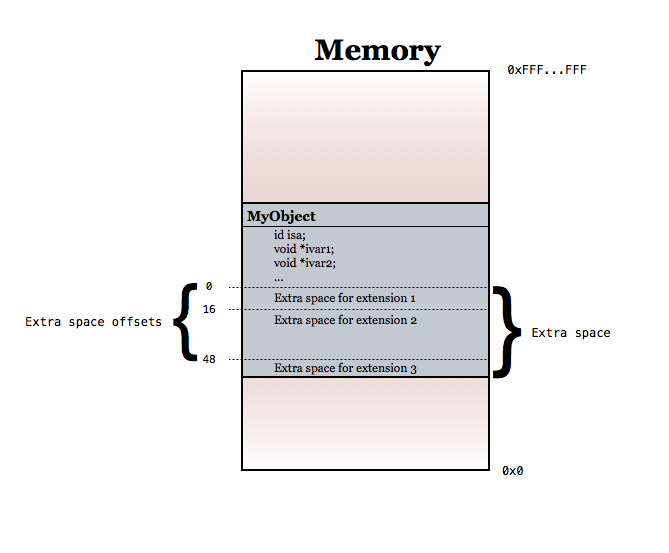
\includegraphics[width=\textwidth]{img/class_extensions.png}
  
  \centering{}
  \caption{Example of how class extensions use memory within an object.}
  \label{fig:class_ext_mem_usage_img}
\end{figure}

There are two examples bundled with the run-time: associated objects (see \verb=extras/ao-ext.c=) and categories (see \texttt{extras/categs.c}). Both examples are discussed below the subsection on Performance (subsections \ref{associated_objects_example_1} and \ref{associated_objects_example_2}).

\textbf{Note:} While changing the fields of the class extension that declare the number of extra bytes required is technically possible, after the first object has been allocated, it will not allocate more space. To speed up object allocation, the sum of extra bytes required is cached. Changing these fields will only result in the class extensions reading (or writing over) other extension's memory, and possibly to unallocated memory altogether.

\subsection{Performance}
Just like anything, even adding class extensions affects the performance somehow. If no extensions are installed in the run-time, the objects are created directly. When extensions get installed, the extension list needs to be iterated and for each extension, one extra function call is performed, if an object initializing function is installed. This iteration itself does not change the asymptotic complexity as the number of class extensions is a constant number, assumed to be a very small one. The only thing that can effect the performance is the object initializer function itself. A quick summary of performance overheads per each function follows.

\begin{itemize}
  \item{\bf{\tt{object\_allocator\_for\_class} and \tt{object\_deallocator\_for\_object}}} The overhead of supplying a custom object allocator and deallocator is at least one function call - the run-time needs to call each extension's (de)allocator lookup until a non-\verb=NULL= (de)allocator is returned. Assuming that there is only one extension that supplies a special allocator depending on the instance size passed as the second argument of this function, the overhead is exactly one function call, plus the logic within that function.
  \item{\bf{\tt{class\_initializer}}} Common frameworks, such as AppKit and Foundation, include roughly 1000 classes each (which can be verified by the aforementioned \verb=objc-dump= tool), 2000 classes altogether, give or take. Which means 2000 function calls to an initializer for each class extension - per run. As has been mentioned, all of the initialization should be lazy, if possible.
  \item{\bf{\tt{object\_initializer}}} Whenever an object is created, each class extension is given the opportunity to initialize its extra space. Again, all of the initialization should be lazy, if possible, as there may be many objects allocated that will not take advantage of that particular class extension.
  \item{\bf{\tt{object\_destructor}}} Calling an object destructor is again only calling a function for each class extension. Assuming that number of class extensions is a small and constant number, one can compare such calls to releasing instance variables within the \texttt{dealloc} method - each class extension implementing the destructor would represent one variable.
  \item{\bf{\tt{instance\_lookup\_function} and \tt{class\_lookup\_function}}} These two functions may look like they could present a major slow down as the lookup function should be as fast as possible. This would be true, if the caching mechanism were not in place. As has been described above, the run-time first looks into the cache. And only if the method is not cached, the class extensions are called to look for the implementation, which then gets cached for the next call. So it really is only once per class per method.
\end{itemize}

\subsection{Example 1: Associated Objects}\label{associated_objects_example_1}

Since OS X 10.6, Apple run-time allows to simulate addition of variables to an object using associated objects\cite{associated_objects}. It allows to specify an object for a key (which is \verb=void *=). Simply said, each object has an assigned hash map, where it stores objects.

\paragraph{Apple's implementation}

Apple's implementation relies on the fact that associated objects are not widely used (at least for now) and are more or less used by the OS's frameworks and a few advanced developers. Hence Apple's approach is to create a single hash map, guarded by a spin lock even on a read (indeed a spin lock as can be seen in file \verb=objc-references.mm=, line 195). Not to mention that it's a subclass of a C++ class \verb=unordered_map=, which then contains a hash map of the associated objects for each object (a subclass of the C++ \verb=std::map=). 

The first time one wants to store an associated object, a new hash map is created for that object and the associated object is then stored in it. When the object is deallocated, the run-time looks into the map and removes all entries for that object.

This solution is sufficient, unless the associated objects get to be used more commonly - having a million objects, each having some associated objects, means a million entries in the object hash map and a million hash maps stored in it. Not to mention that every access is guarded by a spin lock.

\paragraph{Modular run-time implementation}

The solution that is included with this run-time as an 'extra' has been included mainly to demonstrate the class extension capabilities, not to implement the whole associated objects API - for example, the retention policy, which lets the user retain objects as they are set as associated is not implemented, however, adding such a capability is nothing difficult.

The approach that has been chosen is to lazily allocate a small hash map directly on each object and to deallocate it as the object is being deallocated.

With the class extensions, it is fairly easy to achieve. The class itself does not need to be modified at all, hence the \verb=class_initializer= may be \verb=NULL= and \verb=extra_class_space= should be set to 0.

The \verb=extra_object_space= can be set to \verb=sizeof(void *)= in case the hash-table structure should get allocated dynamically, or something else, if it is desired to inline the structure.

If the dynamically allocated hash-table should be used, the \newline{}\verb=object_initializer= can be \verb=NULL= as well and the \verb=object_deallocator= should simply deallocate the hash-table structure if it were ever created.

The \verb=instance_lookup_function= may be \verb=NULL= as well, unless some Objective-C interface should be automatically provided, for example, methods \newline{}\verb=associatedObjectForKey:= and \verb=setAssociatedObject:forKey:= - even that is possible.

Then some getter and setter functions for associated objects can be created. To access the hash-table from an \verb=id object=, code similar to the example shown in figure ~\ref{fig:class_ext_ao} can be used.

\begin{figure}[H] 
\begin{verbatim}
  
  // It is much easier to pretend that
  // the space on the object is really
  // a structure with a single pointer
  // as can be seen later.
  typedef struct {
    ao_bucket **buckets;
  } ao_extension_object_part;
  
  // Static declaration of the extension
  static objc_class_extension 
      associated_objects_extension = { ... }

  // At the beginning, the extension gets added to the run-time
  objc_class_add_extension(&associated_objects_extension);

  // Hash table is retrieved
  ao_extension_object_part *ext_part = 
        objc_object_extensions_beginning_for_extension(obj, 
                                                      &ao_extension)

  // Technically as the offset is 0,
  // buckets == ext_part, but it is
  // a cleaner solution, mainly if
  // you need more variables stored.
  ao_bucket *buckets = ext_part->buckets;
        
  // Do something with the buckets
\end{verbatim}
  \centering{}
  \caption{Example of a class extension - associated objects.}
  \label{fig:class_ext_ao}
\end{figure}


Very similarly, properties could be implemented, with the addition of storing the declared properties in the class structure (i.e.\ \verb=extra_class_space= would be non-zero), however, in the traditional run-time, the properties themselves are just meta data with the actual backing store in ivars - it does not really make much sense to add a property without a link to an ivar, unless it's dynamic (i.e.\ resolved using method calls dynamically), simply because there is nowhere to store it. This is why properties can be added to a class that has already been registered with the run-time (is not in construction), because adding a property does not change the instance sizes.

This way the properties could actually be stored in a separate storage, making it less memory efficient, yet more flexible - it would allow adding variables to a class when it has already been finished/registered with the run-time, allowing a JavaScript-like behavior, adding variables on the fly.

\subsection{Example 2: Categories}\label{associated_objects_example_2}

Categories are a way of adding methods (both class and instance) to existing classes that may even be implemented in a completely different binary. It is a way of extending classes as well as overriding their behavior, since class categories have a priority when it comes to looking up a method implementation.

The traditional run-times tie the categories tightly with the classes, the modular run-time separates them into a class extension.

The whole logic behind the class categories, thanks to the simplicity of class extensions fits into less than 200 lines of code. What is really needed by the extension?

\begin{itemize}
  \item{\bf{Ability to add categories to classes}} This can be simply achieved by requiring extra space on the class structure of size \verb=sizeof(objc_array)= - a single pointer, an array that will hold the list of categories. And some additional interface for doing so, e.g. \verb=objc_class_add_category=.
  \item{\bf{Altering the look-up mechanism}} The class extensions allow adding look up functions that may override the default look-up mechanism. Adding two functions that look through the class' methods and returns one if can be found is all that is necessary.
\end{itemize}

An example of the categories is included with the run-time in \verb=extras/=\newline{}\verb=categs.c=.

\section{Class Prototypes}

The run-time uses prototype structures that can be seen in figure ~\ref{fig:objc_prototypes}.

\begin{figure}[H]
  \begin{verbatim}
    struct objc_method_prototype {
      const char *selector_name;
      const char *types;
      IMP implementation;
      unsigned int version;
    };
    
    
    struct objc_class_prototype {
      Class isa; /* Must be NULL! */
      const char *super_class_name;
      const char *name;
	
      /** All must be NULL-terminated. */
      struct objc_method_prototype **class_methods;
      struct objc_method_prototype **instance_methods;
      Ivar *ivars;
	
      /* Cache - all pointers must be NULL */
      objc_cache class_cache;
      objc_cache instance_cache;
	
      unsigned int instance_size; /* Will be filled */
      unsigned int version; /** Right now 0. */
      struct {
        BOOL in_construction : 1; /* Must be YES */
      } flags;
      
      void *extra_space; /* Must be NULL */
    };
  \end{verbatim}
  \centering{}
  \caption{Structures used as prototypes for class and method declarations.}
  \label{fig:objc_prototypes}
\end{figure}

The method prototype is quite self explanatory. The run-time only replaces the selector name with a real selector. Notice that the prototypes match their real structures, which means all operations may be performed in place, without copying the structure anywhere.

The class prototype probably needs a little explanation. The \verb=isa= pointer must be \verb=NULL=. This is to detect if someone tried to pass a finished \verb=Class= as the prototype. The name of the superclass gets replaced by a pointer to the superclass, if such a class exists. If not, the prototype is ignored.

Class method and instance method prototypes get simply transformed into an array of \verb=Method= pointers, which gets added into an instance of \verb=objc_array=. Similarly, the \verb=ivars= field gets replaces by \verb=objc_array=, into which all ivars are added.

Instance size may be whatever number since it gets replaced during the ivar transformation, when the run-time computes the instance size depending on the superclass' instance size and ivars the class lists.

The version number denotes the version of the class structure to ensure backward compatibility, if it were to change. This is also why the function registering a class prototype returns a \verb=Class= pointer, which \emph{should} be the same as the pointer of the prototype, however, may differ if any version migration were to be performed.

\section{Internal Classes}

While it is technically not a necessity to include some basic classes with the run-time, it turns out as useful at least.

Both traditional run-times implement a basic object class - \verb=Object=, which is now deprecated by Apple and not known to be widely used altogether.

In the latest versions, however, Apple has started moving the \verb=NSObject= class from the Foundation framework into the run-time library as the tight connection between the run-time and a root class (again, reminding that this is not the only root class, but the most commonly used) can bring some performance improvements.

In particular, the \verb=retain= and \verb=release= methods are implemented in most cases only on the root class - \verb=NSObject=. This way, in Apple's run-time, each class marks whether it has implemented its own retain/release methods and if it hasn't, the run-time may directly invoke the retain/release implementation without even looking into the cache, or climbing up the class hierarchy, looking for a method that is certainly at the root of the tree. Most importantly, these two methods are one of the most frequently used methods - Apple supports a so-called vtable, a set of 16 \verb=IMP= functions that are used the most - the default list can be viewed in figure ~\ref{fig:vtable_def_sels} - comments where such methods are usually implemented have been added.

\begin{figure}[H]
  \begin{verbatim}
    static const char * const defaultVtable[] = {
      "allocWithZone:", /** +NSObject, allocating objects. */
      "alloc", /** +NSObject, allocating objects. */
      "class", /** -NSObject, getting class of an object. */
      "self", /** -NSObject, returning self. */
      "isKindOfClass:", /** +NSObject, detecting subclasses. */
      "respondsToSelector:", /** +-NSObject, message sending. */
      "isFlipped", /** -NSView, whether the view is flipped. */
      "length", /** -NSString, length of a string. */
      "objectForKey:", /** -NSDictionary, getting members. */
      "count", /** -NSArray, number of objects. */
      "objectAtIndex:", /** -NSArray, object at index. */
      "isEqualToString:", /** -NSString, equality. */
      "isEqual:", /** -NSObject, equality. */
      "retain", /** -NSObject, memory management. */
      "release", /** -NSObject, memory management. */ 
      "autorelease", /** -NSObject, memory management. */
    };
  \end{verbatim}
  \centering{}
  \caption{Default list of vtable selectors in Apple's run-time.}
  \label{fig:vtable_def_sels}
\end{figure}

The idea behind is similar to what has been described in Chapter 1 - each class has a vtable and if any of the methods is implemented on that class, that slot gets filled. This means that calling any of the methods listed above is as fast as a C function call since the run-time only reaches to a particular slot in the vtable.

The reference counting related methods are indeed included and so are many methods on \verb=NSObject=.

\subsection{MRObject}

The run-time hence includes a basic object class called \verb=MRObject= (\verb=MR= standing for Modular Run-time). While it does not implement all methods implemented by \verb=NSObject=, it implements the basic methods for creating the object (\verb=alloc=) and reference counting \verb=retain= and \verb=release= methods.

\paragraph{Reference counting in traditional run-times} With reference counting, an interesting question pops up - where to store the reference count? How come \verb=NSObject= only has one ivar \verb=isa=? The answer is that the reference count for each object is stored in an external structure (even though in \verb=objc-internal.h= is a macro that would implement the retain/release methods using an ivar). This has two sides:
\subparagraph{Upsides}
\begin{itemize}
  \item{\bf{Hidden from the user}} A regular user (developer) cannot access the reference count directly, which in general is a good thing, however, when someone wants to implement their own reference counting, he or she adds a \verb=referenceCount= ivar to his or her class anyway and there is no good reason to temper with the variable, since it would most likely cause the application to crash very soon.
  \item{\bf{Code reuse}} As the retain count is not a part of any particular class, all classes, even classes without inheriting from \verb=NSObject= may use this mechanism (there are functions exported from the Foundation framework which allow increasing and decreasing reference count for an object - any object).
  \item{\bf{Saving memory when using GC}} As garbage collection completely ignores the reference counting system, the reference counting hash map does not need to be created and as there is no ivar on the \verb=NSObject= that would contain the reference count, memory is saved. This advantage has, however, very low weight since GC is deprecated.
\end{itemize}
\subparagraph{Downsides}
\begin{itemize}
  \item{\bf{Spin lock}} The structure for accessing the structure with reference counts is guarded by a spin lock, slowing down parallel retaining and releasing, even of different objects.
  \item{\bf{Memory usage}} Even though when using garbage collection, some memory may be saved, in other cases, more memory is used than if an ivar were used since some memory is needed for the hash table structure, each entry in the structure needs to remember the object pointer and reference count.
\end{itemize}
\subparagraph{Possible solutions}
\begin{itemize}
  \item{\bf{Make the reference count an ivar}} Of course, this would solve both the spin lock and memory issues, since atomic swap and increment can be used to modify the reference count ivar. Unfortunately, if this were to be a solution for the \verb=NSObject= class in particular, it would bring up many issues with backward compatibility.
  \item{\bf{A hidden reference count ivar}} This could be solved using a hidden ivar that would be ``in front" of the actual object. While the function \verb=class_createInstance= would allocate memory at address \verb=X=, it would return an address \verb=X + sizeof(int)= (note that it should be a signed integer type since an unsigned could underflow into high numbers, making it undetectable), or similar, and the reference count variable would be at address \verb=X=. See figure ~\ref{fig:ref_cnt_hidden_ivar} for a diagram. This could be an issue with statically created objects, like constant strings, however, these objects usually have the retain and release methods overridden to do nothing, their reference count being the maximum integer of that size possible. Of course, it would require all objects to be created using the run-time function for creating instances.
\end{itemize}

\begin{figure}[H]
  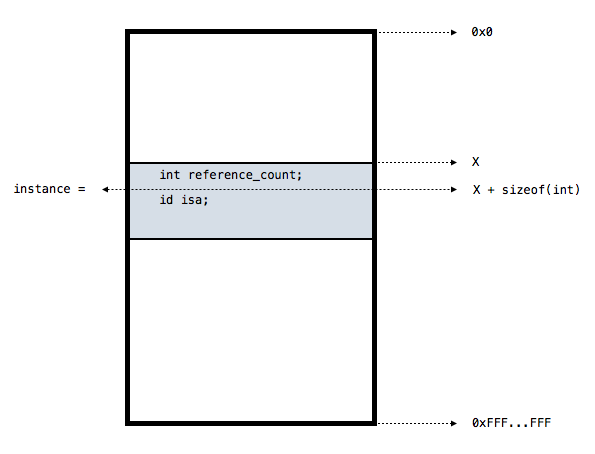
\includegraphics[width=\textwidth]{img/hidden_ref_cnt_var.png}
  
  \centering{}
  \caption{Diagram of a hidden reference count variable.}
  \label{fig:ref_cnt_hidden_ivar}
\end{figure}

\verb=MRObject=, on the other hand gets a fresh start since there are no dependencies on it and hence the \verb=MRObject= class indeed has a reference count variable.

\subsection{\_\_MRConstString}

Strings are one of the most commonly used data types as they are the core for interaction with humans. This is why C has string literals (arrays of chars) and Objective-C has them as well.

Since in order for a piece of memory to validate as an Objective-C object, it must be a pointer to a structure whose first field is an \verb=isa= pointer, a C string literal does not pass for an object. Therefore, the \verb=@"String"= has been introduced. Such a string not only results in a constant C string, but also a static object declaration.

The \verb=__MRConstString= inherits from \verb=MRObject= and adds a single variable - the C string. Simply implementing a class is not enough, however, since the question is how to create the static variables of the class. The \verb=__MRConstString= instance has altogether 3 variables - the isa pointer, the retain count and the C string itself.

The C string itself is quite easy - it's a pointer to a C string literal. The retain count can be set to 1, or really whatever, since the class overrides the retain and release methods to no-op.

The question with creating static Objective-C variables is getting the isa pointer, since you can only use compile-time variables, hence cannot use the \verb=objc_class_for_name= function, or any other run-time related functions.

The solution to this is to export a class prototype structure as can be seen on figure ~\ref{fig:mr_const_str_export}.

\begin{figure}[H]
  \begin{verbatim}
    /** In the header file. */
    extern struct objc_class_prototype __MRConstString_class;
    
    /** In the source file. */
    struct objc_class_prototype __MRConstString_class = {
      NULL, /** isa pointer gets connected when registering. */
      "MRObject", /** Superclass */
      "__MRConstString",
      NULL, /** Class methods */
      __MRConstString_instance_methods, /** Instance methods */
      __MRConstString_ivars, /** Ivars */
      NULL, /** Class cache. */
      NULL, /** Instance cache. */
      0, /** Instance size - computed from ivars. */
      0, /** Version. */
      {
        YES /** In construction. */
      },
      NULL /** Extra space. */
    };
  \end{verbatim}
  \centering{}
  \caption{\_\_MRConstString class export.}
  \label{fig:mr_const_str_export}
\end{figure}

Since the prototype is exported, which is the same as the future class, since the prototype is only modified to become a real class, \verb=&__MRConstString_class= can actually be placed in place of the isa pointer and everything works out. The run-time comes with a macro for creating such structures - see figure ~\ref{fig:mr_const_str_creation}.

\begin{figure}[H]
  \begin{verbatim}
   #define OBJC_STRING(VAR_NAME, STR) \
         static __MRConstString_instance_t VAR_NAME##_stat_str = 
                             { \
                               (Class)(&__MRConstString_class), \
                               1, \
                               STR \
                             };\
         VAR_NAME = (id)&VAR_NAME##_stat_str;


   /** ... */
   
 
   id myString;
   OBJC_STRING(myString, "Hello world!");
   \end{verbatim}
  \centering{}
  \caption{\_\_MRConstString static instance creation.}
  \label{fig:mr_const_str_creation}
\end{figure}


